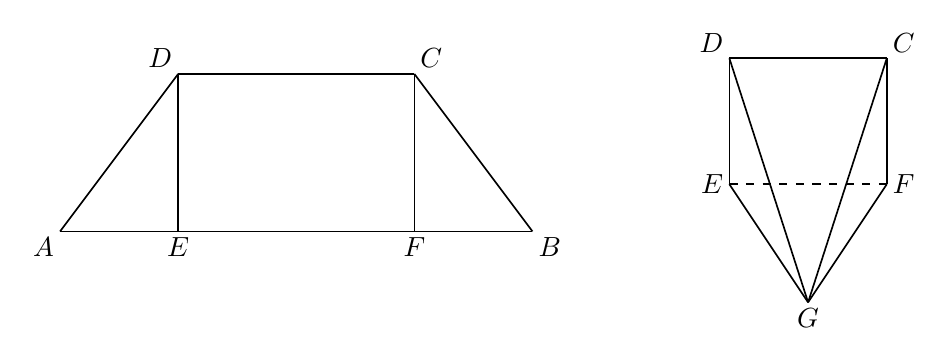
\begin{tikzpicture}[x=1cm,y=1cm,font=\normalsize,
  geometry edge/.style={solid,line width=.6pt},
  geometry label/.style={font=\normalsize,inner sep=2pt}]
% left panel: trapezoid ABCD with altitudes
\coordinate (LA) at (-1.5,0);
\coordinate (LE) at (0,0);
\coordinate (LF) at (3,0);
\coordinate (LB) at (4.5,0);
\coordinate (LD) at (0,2);
\coordinate (LC) at (3,2);
\draw[geometry edge] (LA)--(LE)--(LF)--(LB);
\draw[geometry edge] (LD)--(LC);
\draw[geometry edge] (LA)--(LD);
\draw[geometry edge] (LC)--(LB);
\draw[geometry edge] (LD)--(LE);
\draw[geometry edge] (LC)--(LF);
\node[geometry label,below left] at (LA) {$A$};
\node[geometry label,below] at (LE) {$E$};
\node[geometry label,below] at (LF) {$F$};
\node[geometry label,below right] at (LB) {$B$};
\node[geometry label,above left] at (LD) {$D$};
\node[geometry label,above right] at (LC) {$C$};
% right panel: folded solid CDEFG
\coordinate (RD) at (7,2.2);
\coordinate (RC) at (9,2.2);
\coordinate (RE) at (7,0.6);
\coordinate (RF) at (9,0.6);
\coordinate (RG) at (8,-0.9);
\draw[geometry edge] (RD)--(RC);
\draw[geometry edge] (RD)--(RE);
\draw[geometry edge] (RC)--(RF);
\draw[geometry edge,dashed] (RE)--(RF);
\draw[geometry edge] (RD)--(RG);
\draw[geometry edge] (RC)--(RG);
\draw[geometry edge] (RE)--(RG);
\draw[geometry edge] (RF)--(RG);
\node[geometry label,above left] at (RD) {$D$};
\node[geometry label,above right] at (RC) {$C$};
\node[geometry label,left] at (RE) {$E$};
\node[geometry label,right] at (RF) {$F$};
\node[geometry label,below] at (RG) {$G$};
\end{tikzpicture}
